\section{A sharp conditional-purity bound}
\label{sec:conditional}

The previous continuity classification identifies every singular point.
We can also determine exactly how large the jump can be at each point.
The key is a sharp bound involving a single rank-one conditional state.

\begin{theorem}[Sharp invariant conditional-purity bound]\label{thm:conditional}
Suppose an Alice rank-one projection, of positive probability, prepares
a normalized Bob state $\sigma$ with Bloch-vector length $r\in[0,1]$.
Define
\begin{equation}\label{eq:conditionalcap}\boxed{
 M(r)^2=1+\frac{(1+3r)^2}{3+6r-r^2}.}
\end{equation}
Then
\begin{equation}\label{eq:conditionalbound}
 \HF_A(\rho)\leq M(r).
\end{equation}
The function $M$ is strictly increasing, with
$M(0)=\sqrt{4/3}$ and $M(1)=\sqrt3$. The bound is sharp for every $r$.
\end{theorem}
\begin{proof}
Rotate Alice's projection to $|0\rangle$ and Bob's conditional state to
$\sigma=\diag(\alpha,\beta)$, where
$\alpha=(1+r)/2$ and $\beta=(1-r)/2$.
Write the density matrix in Alice blocks as
\[
 \rho=\begin{pmatrix}A&C\\C^\dagger&B\end{pmatrix},
 \qquad A=t\sigma,\quad \tr B=1-t,\quad0<t\leq1.
\]
The two-qubit purity identity gives the exact expression
\begin{align}\label{eq:blockidentity}
 F_3(\rho)^2={}&8\tr(CC^\dagger)-4|\tr C|^2
 +2\tr(A^2)+2\tr(B^2)-4\tr(AB)-(2t-1)^2.
\end{align}
For clarity, this follows by substituting the block expressions into
$F_3^2=4\tr(\rho^2)-1-\norm a^2-\norm b^2$:
$\norm a^2=(2t-1)^2+4|\tr C|^2$ and
$\norm b^2=2\tr[(A+B)^2]-1$.

Factor the positive matrix as
$\rho=\binom XY\binom XY^\dagger$, so that
$A=XX^\dagger$, $C=XY^\dagger$ and $B=YY^\dagger$.
Then
$\tr(CC^\dagger)=\tr[(X^\dagger X)(Y^\dagger Y)]
\leq\norm{X^\dagger X}_{\rm op}\tr(Y^\dagger Y)
=\norm A_{\rm op}\tr B=t\alpha(1-t)$.
This argument includes singular blocks without taking inverses.
Also $\tr(B^2)\leq(1-t)^2$,
$\tr(AB)\geq t\beta(1-t)$, and
$\tr(A^2)=t^2(1+r^2)/2$.
Applying these inequalities in \eqref{eq:blockidentity} yields
\begin{align}\label{eq:conditionalparabola}
 F_3(\rho)^2
 &\leq1+(2+6r)t-(3+6r-r^2)t^2\\
 &=M(r)^2-(3+6r-r^2)
       \left(t-\frac{1+3r}{3+6r-r^2}\right)^2.\nonumber
\end{align}
The denominator is positive on $[0,1]$, proving the bound for the
unfiltered state.

It remains to prove the asserted filtering invariance. If the initial
projection vector is $|v\rangle$ and $K$ is invertible, project the filtered
state onto a normalized vector proportional to $K^{-\dagger}|v\rangle$.
The resulting Bob state is the same $\sigma$, because the two factors
of $K$ cancel before normalization. It has positive probability.
Thus the preceding unfiltered bound applies to every invertibly filtered
state; taking its supremum proves \eqref{eq:conditionalbound}.

For sharpness put $t_*=(1+3r)/(3+6r-r^2)$ and take
\begin{align}\label{eq:sharpconditional}
 \rho_*={}&t_*\alpha|00\rangle\langle00|
 +t_*\beta|01\rangle\langle01|
 +(1-t_*)|11\rangle\langle11|\nonumber\\
 &+\sqrt{t_*\alpha(1-t_*)}
      (|00\rangle\langle11|+|11\rangle\langle00|).
\end{align}
This is a positive trace-one matrix: its $00,11$ block has determinant
zero and nonnegative diagonal entries, and its remaining nonzero entry
is $t_*\beta\geq0$. Every bound used above is an equality, and
postselection on $|0\rangle$ gives $\sigma$.
Therefore $F_3(\rho_*)=\HF_A(\rho_*)=M(r)$.
Finally direct differentiation gives
\[
 \frac{d}{dr}M(r)^2=
 \frac{4(1+3r)(3+5r)}{(3+6r-r^2)^2}>0,
\]
proving the monotonicity and endpoint values.
\end{proof}

\begin{corollary}[The least pure rank-one conditional state bounds the orbit]
For a mixed Alice marginal define
\[
 r_{\min}=\min_{\norm n=1}
       \frac{\norm{b+T^Tn}}{1+a\cdot n}.
\]
Then $\HF_A\leq M(r_{\min})$. The minimum concerns rank-one projections,
that is, the conditional \emph{surface}. Replacing it by the full
steering-ellipsoid solid is invalid: even a Bell state's solid contains
the origin, while all its rank-one conditional states are pure.
\end{corollary}
\begin{proof}
The denominator is positive and the sphere is compact, so the minimum
exists. Apply Theorem \ref{thm:conditional} to a minimizing projection
and use monotonicity of $M$.
\end{proof}

The sharp family is an amplitude-damping or maximally-obese steering
ellipsoid family after canonicalization. That family is established
quantum-state geometry \cite{milne}; it is not claimed as a new family. The bound,
its equality proof and the cluster-set consequence below are explicit
derivations in this package. A bounded search does not establish their
publication priority.

\section{The exact cluster interval at every pure-marginal state}\label{sec:cluster}

\begin{theorem}[Complete singular cluster set]\label{thm:clusters}
Fix $\rho_0=|u\rangle\langle u|\otimes\sigma$ and let $r$ be the Bloch
length of $\sigma$. The set of limits of $\HF_A(\rho_n)$ along convergent
sequences $\rho_n\to\rho_0$ is exactly
\begin{equation}\label{eq:clusters}\boxed{
 [r,M(r)]=\left[r,\sqrt{1+\frac{(1+3r)^2}{3+6r-r^2}}\right].}
\end{equation}
In particular the lower limit is $r$, the upper limit is $M(r)$,
and the maximal discontinuity jump is exactly $M(r)-r$.
\end{theorem}
\begin{proof}
By local-unitary invariance take $|u\rangle=|0\rangle$ and diagonalize
$\sigma$. Lower semicontinuity already gives a lower bound $r$ on every
cluster value. For states $\rho_n\to\rho_0$, the probability of the
Alice-$0$ projection tends to one, and its normalized Bob state tends
to $\sigma$. Let its Bloch length be $r_n$; then $r_n\to r$ and
Theorem \ref{thm:conditional} gives
$\HF_A(\rho_n)\leq M(r_n)\to M(r)$.

To realize the upper endpoint use $\rho_*$ from
\eqref{eq:sharpconditional}. Apply $D_\epsilon=\diag(1,\epsilon)$ on
Alice and normalize. As $\epsilon\downarrow0$ the state tends to
$|0\rangle\langle0|\otimes\sigma$. For each $\epsilon>0$, the filter
is invertible. The unrestricted quantity is invariant under invertible
filtering on its own side, since composition permutes the group of
all subsequent invertible filters. Every state in this sequence therefore
has value $M(r)$.

For every intermediate value, interpolate
\[
 \omega_s=(1-s)(I/2\otimes\sigma)+s\rho_*,\qquad0\leq s\leq1.
\]
All these states have a mixed Alice marginal and the same normalized
Alice-$0$ conditional Bob state $\sigma$. Thus
$s\mapsto\HF_A(\omega_s)$ is continuous by
Theorem \ref{thm:continuitylocus}. Its endpoint values are $r$ and $M(r)$.
The intermediate value theorem supplies any prescribed value between
them. Fix that $s$ and apply the collapsing filters $D_\epsilon$.
The states converge to $\rho_0$, while invertible-filter invariance
preserves the prescribed value for every $\epsilon>0$.
This realizes the entire interval and proves equality.
\end{proof}

\begin{corollary}[Rigidity of the maximal one-sided value]\label{cor:bellrigidity}
For an arbitrary two-qubit density matrix,
\[
 \HF_A(\rho)=\sqrt3
 \quad\Longleftrightarrow\quad
 \rho\text{ is a pure entangled state}
 \quad\Longleftrightarrow\quad
 \HF_B(\rho)=\sqrt3.
\]
\end{corollary}
\begin{proof}
An entangled pure state can be converted invertibly to a Bell state by
Schmidt concentration. Conversely $\sqrt3>1$, so the main theorem's
violating-branch result guarantees an attained invertible optimizer.
Its output has $F_3^2=3$. The identity
\[
 4\tr(\rho_{\rm out}^2)=1+\norm{a_{\rm out}}^2
             +\norm{b_{\rm out}}^2+F_3(\rho_{\rm out})^2
\]
and $\tr(\rho_{\rm out}^2)\leq1$ force zero marginal Bloch vectors and
purity one, hence a Bell state up to local unitaries. An invertible
filter preserves matrix rank, so the input is pure. It cannot be a
product state, whose filtered value is at most one.
\end{proof}

\begin{proposition}[An explicit global modulus at fixed success rate]
\label{prop:globalmodulus}
For $0<p<1$ and $\Delta=\norm{\rho-\sigma}_1$,
\begin{equation}\label{eq:globalmodulus}
 |\HF_A(\rho;p)-\HF_A(\sigma;p)|
 \leq\frac{2\sqrt3}{p}
 \left(\Delta+2\sqrt{\frac{\Delta}{1-p+\Delta}}\right).
\end{equation}
At $p=1$ the sharper bound is $\sqrt3\,\Delta$. The same statements hold
for Bob. Thus the fixed-rate regularization is quantitatively uniform
over all density matrices, without a lower bound on marginal eigenvalues.
\end{proposition}
\begin{proof}
Take a maximizing $\rho$-feasible filter $K=U\sqrt E$, and set
$t=\Delta/(1-p+\Delta)$,
$E_t=(1-t)E+tI$, $K_t=U\sqrt{E_t}$.
Trace-norm duality gives success on $\sigma$ at least
$(1-t)(p-\Delta)+t=p$.
Since $E_t$ commutes with $E$ and their eigenvalues lie in $[0,1]$,
$\norm{K_t-K}_{\rm op}\leq\sqrt t$.
The two unnormalized output matrices then differ in trace norm by at
most $\Delta+2\sqrt t$, using the contraction property and a two-term
expansion in $K_t-K$. Normalizing matrices of trace at least $p$ increases
this bound by at most $2/p$.

Finally $|F_3(\omega)-F_3(\omega')|\leq
\sqrt3\norm{\omega-\omega'}_1$. To verify the constant, pair the
correlation difference with a Frobenius-unit real matrix $R$.
An orthogonal singular-value decomposition gives
$\norm{\sum_{ij}R_{ij}\sigma_i\otimes\sigma_j}_{\rm op}
\leq\sum_i s_i(R)\leq\sqrt3$; trace-norm duality and Frobenius-norm
duality give the assertion. Applying it to the two normalized outputs
gives one direction of \eqref{eq:globalmodulus}. Interchange $\rho$ and
$\sigma$ for the other. At $p=1$, both optimized values equal the
unfiltered $F_3$, so the last Lipschitz estimate applies directly.
\end{proof}

\begin{figure}[htbp]
\centering
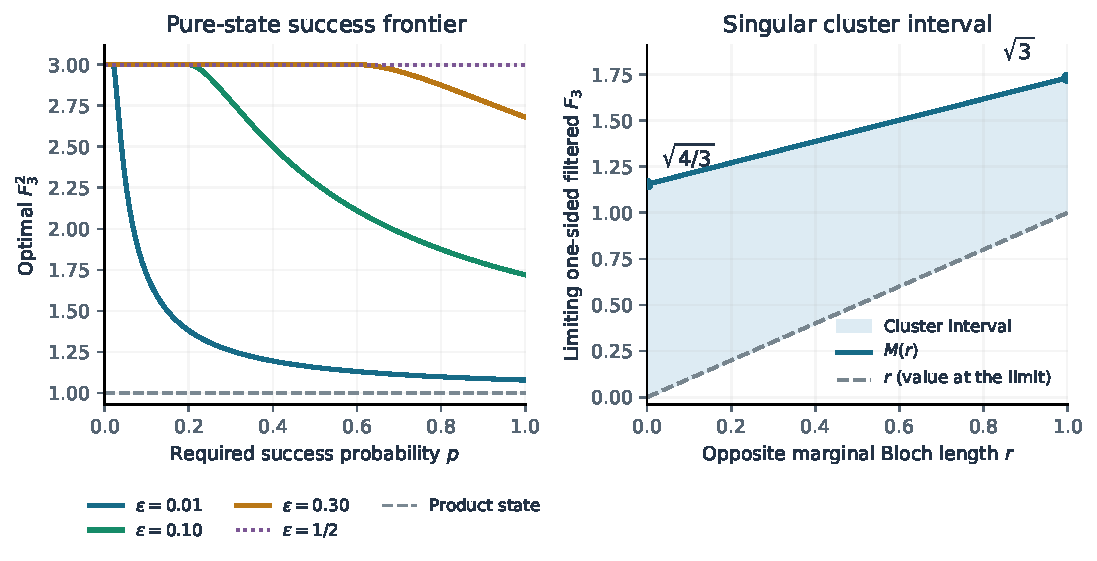
\includegraphics[width=\textwidth]{figures/operational_frontiers.pdf}
\caption{Exact analytical curves, without numerical filter optimization.
Left: the pure-state frontier in Theorem \ref{thm:purefrontier}; its Bell plateau
ends at $p=2\varepsilon$. Right: every value in the shaded interval is a cluster
value at the corresponding pure-marginal product state, by
Theorem \ref{thm:clusters}. A fixed positive rate restores continuity across
these singular limits. The figure is reproduced by \texttt{checks/make\_figures.py}.}
\end{figure}
